\chapter{\tool{Coq}的证明可视化}\label{chapt:coqv}

本章工作是作为上一章工作的扩展。
在上一章中我们提到,\tool{VMDV}提供了一个一般化的接口,用于与不同的定理证明工具进行通讯,进而可以实现不同定理证明工具的证明可视化。本章介绍的是对于一个成熟的,并且在工业界以及学术界得到广泛使用的定理证明工具\tool{Coq}的证明可视化。

\section{\tool{Coq}概述}
\couic{The Coq system is designed to develop mathematical proofs, and especially to write formal specifications, programs and to verify that programs are correct with respect to their specification. It provides a specification language named Gallina. Terms of Gallina can represent programs as well as properties of these programs and proofs of these properties. Using the so-called Curry-Howard isomorphism, programs, properties and proofs are formalized in the same language called Calculus of Inductive Constructions, that is a λ
	-calculus with a rich type system. All logical judgments in Coq are typing judgments. The very heart of the Coq system is the type-checking algorithm that checks the correctness of proofs, in other words that checks that a program complies to its specification. Coq also provides an interactive proof assistant to build proofs using specific programs called tactics.

Coq has an interactive mode in which commands are interpreted as the user types them in from the keyboard and a compiled mode where commands are processed from a file.

The interactive mode may be used as a debugging mode in which the user can develop his theories and proofs step by step, backtracking if needed and so on. The interactive mode is run with the coqtop command from the operating system (which we shall assume to be some variety of UNIX in the rest of this document).
The compiled mode acts as a proof checker taking a file containing a whole development in order to ensure its correctness. Moreover, Coq’s compiler provides an output file containing a compact representation of its input. The compiled mode is run with the coqc command from the operating system.
}
\tool{Coq}是一个计算机辅助定理证明工具。研究人员和工程人员利用\tool{Coq}可以开发程序,并表达程序的规范,然后利用定理证明的方式来形式化验证程序是否满足规范。因此,\tool{Coq}适合开发需要绝对可信的程序,这样的程序在许多行业中是非常重要的,比如航空航天、交通以及银行等。\tool{Coq}通常以交互的方式来构造证明,并尽可能利用自动化的证明搜索工具的辅助。\tool{Coq}不仅可以作为一个形式化验证系统,还可以作为一个逻辑框架来为新的逻辑提供公理、定义规则,并基于此来开发证明。

作为一个计算机工具,\tool{Coq}与编程人员交互时需要用到两种语言:Gallina语言和Vernacular语言。Gallina是一个面向表达式的语言,利用Gallina语言的表达式可以来描述项、类型、证明以及程序;Vernacular是一个面向命令的语言,利用Vernacular命令可以控制\tool{Coq}的行为(比如搜索、类型检查以及计算等。),配置\tool{Coq}的参数(比如设置当前工作目录、是否输出警告等),以及最重要的:声明和定义Gallina表达式。\tool{Coq}与编程人员交互的方式是解析编程人员输入的Vernacular命令,并即时反馈解析的结果。


根据柯里-霍华德同构,程序、规范以及证明都可以用归纳构造演算(Calculus of Inductive Construction)\cite{BertotC04}中的项来表示。在归纳构造演算中,所有的逻辑判断(logical judgement)都是类型判断(type judgement),而\tool{Coq}的核心功能即利用类型检查算法来检验证明的正确性,即检查一段程序是否符合其规范。除此之外,\tool{Coq}还提供了一种被称为证明策略(tactic)的机制来构造证明。

\tool{Coq}提供了两种构造证明的模式:交互模式和编译模式。
\begin{itemize}
	\item 交互模式:用户通过在操作系统的命令行中输入“coqtop”来开启交互模式。
	在这种模式中,用户可以通过逐步输入命令的方式来构造理论和证明。
	\item 编译模式:用户通过在操作系统的命令行中输入“coqc”来调用\tool{Coq}的编译模块。编译模块可被看作为证明检查工具,并来确保所输入的文件中包含的Vernacular命令是正确的。
\end{itemize}

\subsection{\tool{Coq}的用户接口}
\tool{Coq}的用户接口的作用是辅助用户编写Vernacular命令,并实时显示\tool{Coq}对命令的解析状态,反过来帮助用户完成余下的命令的编写。目前最常用的\tool{Coq}用户接口为\tool{Proof General}\footnote{\url{https://proofgeneral.github.io}}和\tool{CoqIDE}\footnote{\url{https://github.com/coq/coq/wiki/CoqIde}}。\tool{Proof General}是一个基于Emacs\footnote{\url{https://www.gnu.org/software/emacs/}}的定理证明工具的前端(front end),并提供了一个统一的接口来适配不同的定理证明工具。不同于\tool{Proof General},\tool{CoqIDE}是一个独立的,专门针对\tool{Coq}的图形用户界面系统。
在这两个用户接口程序中都可实现\tool{Coq}的交互和编译两种模式的证明。

\subsection{解析Vernacular命令}
\begin{figure}[h!]
	\centering
	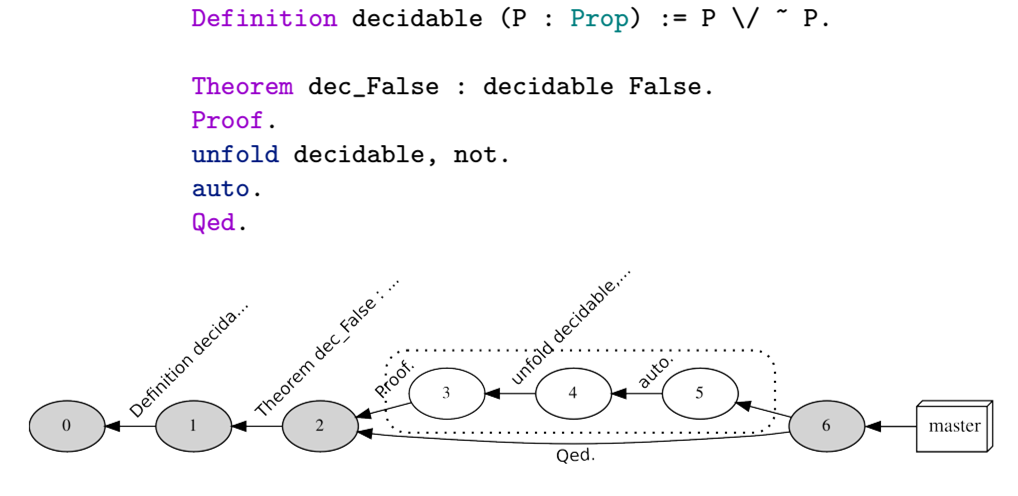
\includegraphics[width=12cm]{Img/coq_stm.png}
	\caption{Vernacular命令以及\tool{Coq}对其的解析}
	\label{coq:stm}
\end{figure}

无论是交互模式还是编译模式,\tool{Coq}都需要对一系列Vernacular命令进行逐个解析。在\tool{Coq}内部有一个被称为系统状态(system state)的概念,\tool{Coq}将每对每条命令的解析看作为从当前的系统状态到下一个系统状态的迁移,当实现回退操作时,系统需要抛弃当前的状态,而重新从上一个状态开始解析命令。自从8.5版本开始,\tool{Coq}利用有向无环图(Directed Acyclic Graph,简称DAG)来记录系统状态:DAG中的点是系统状态,而点与点之间的有向边则标记为一条命令。\tool{Coq}中操作有向无环图的模块被称为状态处理机(State Transaction Machine,简称STM),在STM中,每条命令的解析是自动的、原子的,即命令解析的中间状态是不可见的。
根据作用域的不同,命令可分为两类:局部命令和全局命令。
\begin{itemize}
	\item 局部命令指的是只针对当前的证明起作用的命令。这类命令包括证明策略(证明规则)以及证明处理(开启证明、撤回证明、重启证明、放弃证明、聚焦局部证明、结束证明等)命令。
	\item 全局命令指的是非局部命令。这类命令有:信息显示、设置环境变量、查询环境变量、加载文件、编译文件、设置加载路径、回溯、退出等。
\end{itemize}
例如,在图\ref{coq:stm}中,STM从系统状态0开始依次处理6条命令,每条命令对应着一条有向边,当处理完所有命令后,状态6变为当前的状态(master指针指向的状态)。其中,生成状态1、2、6的命令为全局命令,而生成状态3、4、5的命令为局部命令。




\section{构造与可视化证明树}
\tool{Coq}中的证明可以展现成证明树的形式:每个当前需要证明的命题被称为目标(goal),当应用一条规则,而且该命题匹配当前规则的结论,那么利用与命题和规则的结论同样的匹配方式去例化当前规则的假设,从而得到0个或多个命题,这些新生成的命题被成为子目标(subgoal),然后在新生成的命题上利用相同的证明方式去产生更多的子目标,直到无法生成更多的子目标为止。在这种形式的证明中,每个目标可看作证明树中的一个节点,而其子目标则可看作该节点的子节点。在\tool{Coq}中对一个命题的证明过程则可看作一棵证明树的构造过程,在此过程中所应用的规则即证明脚本中的策略。

然而,无论在\tool{Coq}中,还是在其用户接口\tool{Proof General}和\tool{CoqIDE}中,都不存在构造以及保存证明树的机制,因此这种状况给用户在证明过程中增添了一种无形的负担,即需要自行在脑海中想象当前证明树的完整形状。随着证明操作越来越复杂,比如需要回退操作以及在不同子目标之间相互跳转时等,用户所依赖的信息只有\tool{Coq}给出的当前需要证明的命题的信息,而越来越难以建立起完整的证明树的概念。
为了解决这个问题,我们在本章中研究\tool{Coq}的证明可视化,因此我们设计并开发了一个工具\tool{Coqv}\footnote{\url{https://github.com/ProveVis/coqv}}来完整地记录\tool{Coq}中证明树以及对证明树的操作。\tool{Coqv}通过与\tool{VMDV}结合,就可实现\tool{Coq}的证明树的可视化。

\subsection{\tool{Coqv}的原理}
\begin{figure}[h!]
	\centering
	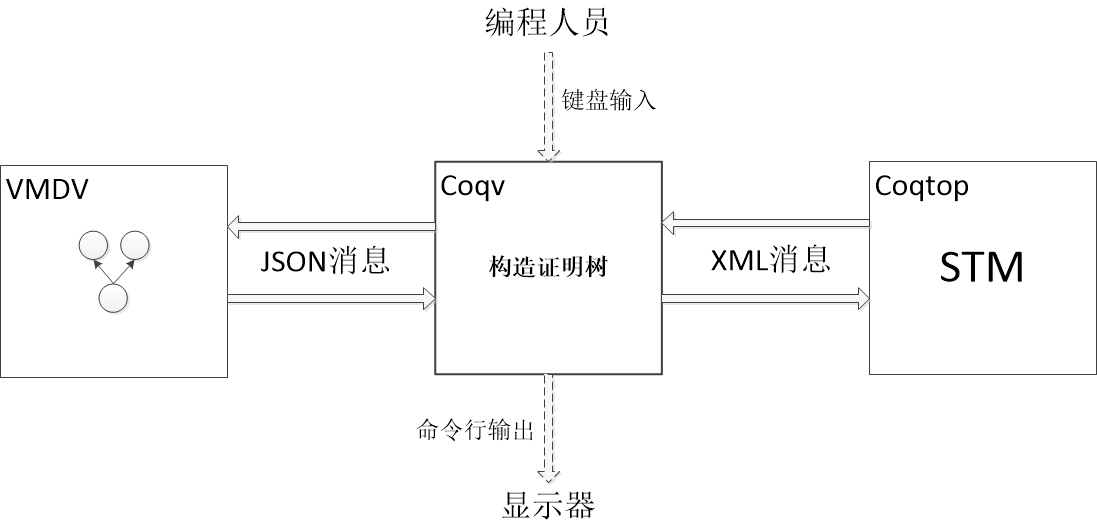
\includegraphics[width=11cm]{Img/coqv_overview.png}
	\caption{\tool{Coqv}作为\tool{VMDV}和\tool{Coqtop}进行通讯的中间件}
	\label{coqv:overview}
\end{figure}
如图\ref{coqv:overview}所示,\tool{Coqv}的作用是作为协调证明可视化工具\tool{VMDV}与\tool{Coqtop}通讯的中间件。
\tool{Coqv}工作流程可总结为:
\begin{enumerate}
	\item \tool{Coqv}接收用户输入的命令,然后将该命令发送到\tool{Coqtop};
	\item \tool{Coqtop}利用STM模块解析所接收到的命令,然后将反馈信息发送给\tool{Coqv};
	\item \tool{Coqv}解析所收到的来自\tool{Coqtop}的反馈消息并在命令行中输出,除此之外,\tool{Coqv}还根据解析的消息内容对证明树进行更新,同时将对于证明树的更新操作发送给\tool{VMDV};
	\item \tool{VMDV}接收到来自\tool{Coqv}的消息,并根据消息内容在3D空间内更新证明树的显示效果,除此之外,用户通过\tool{VMDV}对证明树的操作(比如删除某节点)还可反馈到\tool{Coqv},然后\tool{Coqv}将相应的命令(比如丢弃某个命题的证明)发送给\tool{Coqtop}。
\end{enumerate}

在第1步和第2步中,\tool{Coqv}与\tool{Coqtop}的是通过\tool{Coqtop}内置的XML协议\footnote{\url{https://github.com/siegebell/vscoq/wiki/XML-protocol}}来通讯的;在第3步和第4步中,\tool{Coqv}与\tool{VMDV}是通过\tool{VMDV}内置的JSON协议(见附录\ref{vmdv:json:protocol})来通讯的。

需要注意的是,如果在图\ref{coqv:overview}中去掉\tool{VMDV}相关的部分,则\tool{Coqv}的功能与\tool{Proof General}和\tool{CoqIDE}一致,即都是作为\tool{Coq}的用户接口。因此,相比于其他针对\tool{Coq}的用户接口,\tool{Coqv}增加了构造证明树,以及将证明树的构造信息发送到\tool{VMDV}以进行可视化的功能。

\subsection{在\tool{Coqv}中构造证明树}
在上一小节我们提到,\tool{Coqtop}内置了一个XML协议用来与用户接口进行通讯。该XML协议规定了用户接口向\tool{Coqtop}发送的请求以及\tool{Coqtop}发送给用户接口的反馈。
根据该协议,\tool{Coqv}将要发送的Vernacular命令包装成一个Add请求,其中除了要发送的命令$cmd$之外,一个Add请求还包括当前的系统状态的ID $stateid$以通知STM在当前的状态ID为$stateid$时解析命令$cmd$。如果\tool{Coqtop}成功解析$cmd$命令,则向\tool{Coqv}发送一个反馈,反馈中包括下一个系统状态的ID以及提示信息;如果\tool{Coqtop}解析$cmd$命令失败(即$cmd$有语法错误),也向\tool{Coqv}发送一个反馈,反馈中包含错误信息。
当\tool{Coqv}完成Add请求的发送并收到\tool{Coqtop}的正面反馈后,\tool{Coqv}会根据发送的命令$cmd$的类型来构造证明树。构造方式如下:
\begin{itemize}
	\item 如果$cmd$是一个全局命令,则不更新证明树。这是由于在\tool{Coq}中,一个命题的证明以$Proof.$命令开始,并以$Qed.$结束(当放弃证明的时候以$Admitted.$结束),而且所有这两个命令之间的证明细节对于外部程序是不可见的,只有命题的类型是对外可见的。因此,证明是一个局部的概念,即外部程序只记录命题是否可证,而不记录证明的细节。因此,全局命令无法作用于局部的证明细节,无法影响证明树的构造。
	\item 如果$cmd$是一个局部命令,那么\tool{Coqv}发送一个Goal请求,然后\tool{Coqtop}会返回所有当前的目标(goal),然后\tool{Coqv}根据接收到的当前目标来对证明树进行构造。
	对于不同的局部命令,证明树构造的方式也不一样。
	\begin{itemize}
		\item 对于证明处理命令,如果$cmd$为$Proof.$,那么将当前要证明的命题作为根节点加入证明树中,并将此节点设为焦点;如果$cmd$为$Qed.$,那么结束证明树的构造;如果$cmd$为其他证明处理命令,则本次接收到的所有目标皆已在证明树中存在,那么将这些目标所对应的节点都设为叶子节点,即删除这些节点的所有后代节点,另外,将接收到的第一个目标对应的节点设为焦点。
		\item 对于证明策略,将接收到的所有目标都作为当前焦点节点的子节点加入证明树中,并将接收到的第一个目标对应的节点设为焦点。
	\end{itemize}
\end{itemize}
在\tool{Coqv}发送的所有的命令中,只有证明处理命令$Proof.$和证明策略会对应着产生证明树的新节点,前者对应着证明树的初始化,后者对应着证明树的增长。

\subsection{在\tool{VMDV}中可视化证明树}
